\documentclass[tikz,border=2mm]{standalone}
\usetikzlibrary{shapes,arrows.meta,positioning}
\usepackage{xcolor}
\definecolor{BleuLMS}{RGB}{1, 66, 106}
\definecolor{GreenLMS}{RGB}{0,103,127} % LMPS
\definecolor{LGreenLMS}{RGB}{67,176,42} % LMPS
\definecolor{RougeLMS}{RGB}{206,0,55} % CEA


\tikzstyle{input} = [circle, draw=BleuLMS, fill=BleuLMS!25, minimum size=8mm, thick]

\tikzstyle{inputSpace} = [circle, circular drop shadow, draw=GreenLMS, fill=BleuLMS!25, minimum size=8mm, thick]
\tikzstyle{inputPara} = [circle, circular drop shadow, draw=LGreenLMS, fill=LGreenLMS!25, minimum size=8mm, thick]

\tikzstyle{ShapeF} = [circle, draw=GreenLMS, fill=GreenLMS!25, minimum size=2mm, thick]

\tikzstyle{Sol} = [circle, circular drop shadow, draw=LGreenLMS, fill=LGreenLMS!25, minimum size=2mm, thick]
\tikzstyle{Out} = [circle, circular drop shadow, draw=BleuLMS, fill=GreenLMS!25, minimum size=2mm, thick]
\tikzstyle{Mul} = [circle, circular drop shadow, draw=black, fill=black!25, minimum size=2mm, thick]
\tikzstyle{lineSpace} = [draw,BleuLMS, -,thick]
\tikzstyle{linePara} = [draw,LGreenLMS, -,thick]
\tikzstyle{line} = [draw,GreenLMS, -,thick]
\tikzstyle{lineDot} = [draw,GreenLMS, doted,thick]
\usetikzlibrary {math}
\usetikzlibrary {decorations}
\usetikzlibrary{shadows}

\begin{document}
	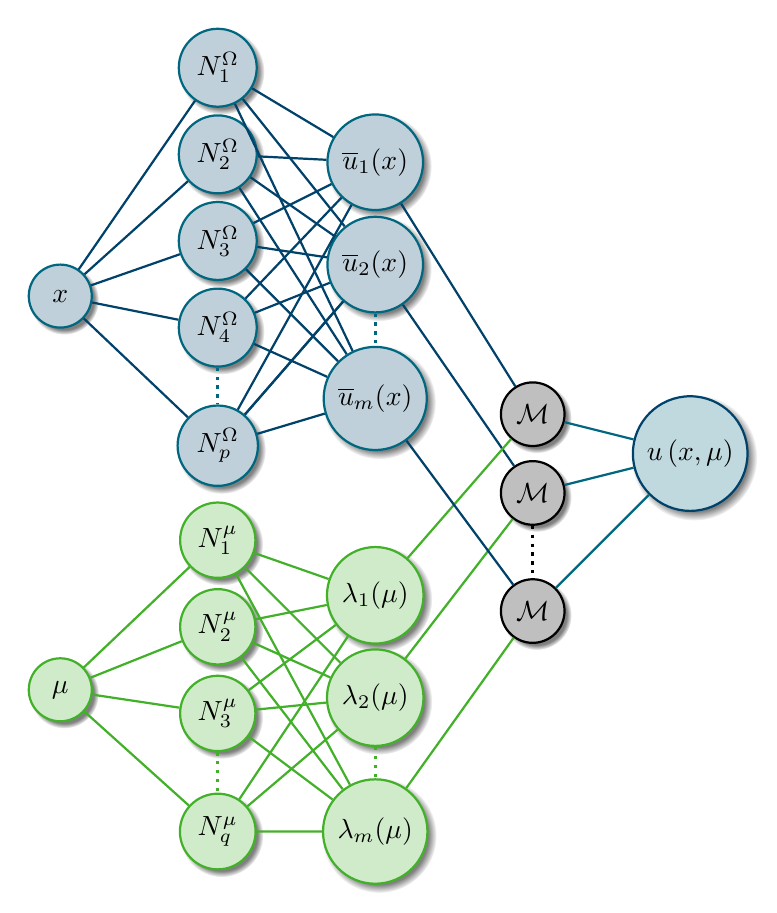
\begin{tikzpicture}[>=Stealth, node distance=1.5cm]

		\def\NN{4} % number of nodes in spatial mesh
		\def\NU{3} % number of nodes in parameter mesh
		\def\NM{2} % number of modes
		

		
		% Input layer
		\foreach \i in {1}
		\node [inputSpace] (I\i) at (0,-1.5-2.5) {$x$};
		
		\foreach \i in {2}
		\node [inputPara] (I\i) at (0,-1-1.5-6.5) {$\mu$};
		
		% Hidden layer
		\foreach \h [count=\hi] in {1,...,\NN}
		\node [inputSpace] (Ho\hi) at (2, -1.1*\h) {$N^{\Omega}_\h$};
		\node [inputSpace] (Last) at (2, -1.1*\NN-1.5) {$N^{\Omega}_p$};
		\draw[dotted, very thick,GreenLMS ] (Ho\NN) -- (Last);
	
		\foreach \h [count=\hi] in {1,...,\NU}
		\node [inputPara] (Hm\hi) at (2, -1.5-4.5-1.1*\h) {$N^{\mu}_\h$};
		\node [inputPara] (Last2) at (2, -1.5-4.5-1.1*\NU-1.5) {$N^{\mu}_q$};
		\draw[ dotted, very thick, LGreenLMS] (Hm\NU) -- (Last2);
		
		% 2nd hidden layer
		\foreach \o [count=\oi] in {1,...,\NM}
		\node [inputSpace] (O\oi) at (4, -1-1.3*\oi) {$\overline{u}_\o(x)$};
		\node [inputSpace] (OLast) at (4, -1-1.3*\NM-1.7) {$\overline{u}_m(x)$};
		\draw[dotted, very thick,GreenLMS ] (O\NM) -- (OLast);
		
		\foreach \o [count=\oi] in {1,...,\NM}
		\node [inputPara] (Om\oi) at (4, -1.5-5-1.3*\oi) {$\lambda_\o(\mu)$};
		\node [inputPara] (OLastm) at (4, -1.5-5-1.3*\NM-1.7) {$\lambda_m(\mu)$};
		\draw[dotted, very thick,LGreenLMS ] (Om\NM) -- (OLastm);
		
		% 3rd hidden layer
		
		\foreach \o [count=\oi] in {1,...,\NM}
		\node [Mul] (Mul\oi) at (6, -1.5-3-\oi) {$\mathcal{M}$};
		\node [Mul] (MulLast) at (6, -1.5-3-\NM-1.5) {$\mathcal{M}$};
		\draw[dotted, very thick,black ] (Mul\NM) -- (MulLast);
		
		%		 output layer
				\node [Out] (Iout) at (8,-1.5-4.5) {$u\left(x,\mu\right)$};
		
		% Connect layers
		\foreach \i in {1}
		\foreach \h in {1,...,\NN}
		\draw [lineSpace] (I\i) -- (Ho\h);
		
		\draw [lineSpace] (I1) -- (Last);
		\draw [linePara] (I2) -- (Last2);
		
		\foreach \i in {2}
		\foreach \h in {1,...,\NU}
		\draw [linePara] (I\i) -- (Hm\h);
		
		\foreach \h in {1,...,\NN}
		\foreach \o in {1,...,\NM}
		\draw [lineSpace] (Ho\h) -- (O\o);
		
		\draw [lineSpace] (Last) -- (O\NM);
		
		\foreach \h in {1,...,\NN}
		\draw [lineSpace] (Ho\h) -- (OLast);
		
		\foreach \h in {1,...,\NM}
		\draw [lineSpace] (Last) -- (O\h);
		
		\draw [lineSpace] (Last) -- (OLast);
		
		\foreach \h in {1,...,\NU}
		\foreach \o in {1,...,\NM}
		\draw [linePara] (Hm\h) -- (Om\o);
		
		\foreach \h in {1,...,\NU}
		\draw [linePara] (Hm\h) -- (OLastm);
		\foreach \h in {1,...,\NM}
		\draw [linePara] (Last2) -- (Om\h);
		
		\draw [linePara] (Last2) -- (OLastm);
		

		\foreach \m in {1,...,\NM}
		\draw [lineSpace] (O\m) -- (Mul\m);
		\foreach \m in {1,...,\NM}
		\draw [linePara] (Om\m) -- (Mul\m);
		
		\draw [lineSpace] (OLast) -- (MulLast);
		\draw [linePara] (OLastm) -- (MulLast);

		
				\foreach \m in {1,...,\NM}
		\draw [line] (Mul\m) -- (Iout);
		
		\draw [line] (MulLast) -- (Iout);
		
%		% Layer labels
%		\node[above=of I1] {Input Layer};
%		\node[above=of Ho1] {Hidden Layer};
%		\node[above=of O1] {Output Layer};
	\end{tikzpicture}
\end{document}
